\documentclass[twoside,twocolumn,8pt]{extarticle}


% ------
% Fonts and typesetting settings
\usepackage[sc]{mathpazo}
\usepackage[T1]{fontenc}
\linespread{1.05} % Palatino needs more space between lines
\usepackage{microtype}


% ------
% Page layout
\usepackage[hmarginratio=1:1,top=10mm,columnsep=20pt,left=0.8in, right=0.8in]{geometry}
\usepackage[font=it]{caption}
\usepackage{paralist}
\usepackage{multicol}

% ------
% Lettrines
\usepackage{lettrine}


% ------
% Abstract
\usepackage{abstract}
	\renewcommand{\abstractnamefont}{\normalfont\bfseries}
	\renewcommand{\abstracttextfont}{\normalfont\itshape}


% ------
% Titling (section/subsection)
\usepackage{titlesec}
\renewcommand\thesection{\Roman{section}}
\titleformat{\section}[block]{\large\scshape\centering}{\thesection.}{1em}{}

\usepackage{graphicx}
% ------
% Header/footer


\usepackage{fancyhdr}
\pagestyle{fancy}

\setlength\headheight{90.0pt}
\addtolength{\textheight}{-90.0pt}

\fancypagestyle{firststyle}
{
   	\fancyhead[L]{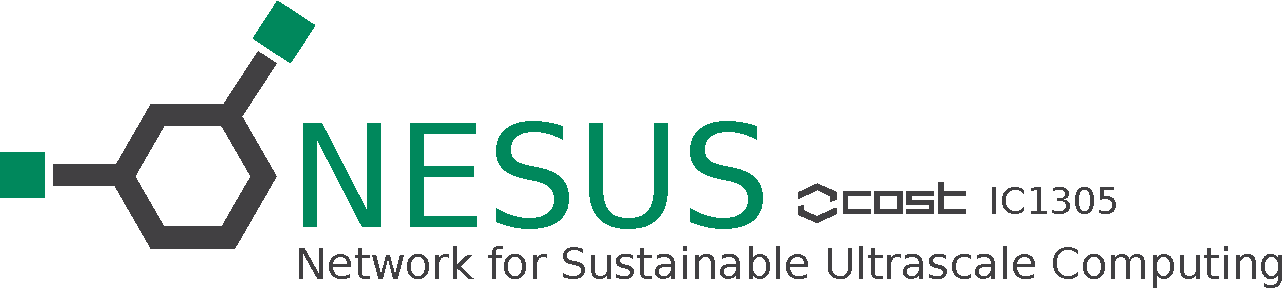
\includegraphics[height=5.5em]{pictures/nesus.pdf}}
	\fancyhead[C]{}
	\fancyfoot{}
	\fancyhead[R]{\small{Book paper template $\bullet$ October 2016 $\bullet$ Vol. I, No. 1}}
	\fancyfoot[RO,LE]{\thepage}
}
	\fancyhead[R]{}
	\fancyhead[L]{}
	\fancyfoot{}
	\fancyhead[C]{\small{Book paper template $\bullet$ October 2016 $\bullet$ Vol. I, No. 1}}
	\fancyfoot[RO,LE]{\thepage}


% ------
% Clickable URLs (optional)
\usepackage{hyperref}

% ------
% Maketitle metadata
\title{\vspace{-10mm}%
	\fontsize{24pt}{10pt}\selectfont
	\textbf{Modeling Emerging Complex Memory Hierarchies With The Roofline Model}
	}
	
		
\author{%
	\large
	\textsc{Nicolas Denoyelle \and Aleksandar Ilic} \\[2mm]
	\normalsize{	Inria - France -- INESC-ID -- Portugal}\\
	\normalsize{	\href{mailto:Nicolas.Denoyelle@inria.fr}{Nicolas.Denoyelle@inria.fr} \href{mailto:ilic@sips.inesc-id.pt}{ilic@sips.inesc-id.pt}}
	\vspace{-5mm}
	}

\date{}

\providecommand{\keywords}[1]{\textbf{\textit{Keywords}} #1}

%%%%%%%%%%%%%%%%%%%%%%%%
\begin{document}



\twocolumn[
  \begin{@twocolumnfalse}

%\maketitle

\thispagestyle{firststyle}


\begin{abstract}
\noindent The ever growing complexity of high performance computing systems imposes significant challenges to exploit as much as
  possible their computational and communication resources.
  Recently, the Cache-aware Roofline Model has has gained popularity due to its simplicity modeling multi-cores with complex memory
  hierarchy, characterizing applications' bottlenecks, and quantifying achieved or remaining improvements.
  In this short paper we push this model a step further to model NUMA and heterogeneous memories with a handy tool, and spot data
  locality bottlenecks on such systems.
\end{abstract}


\keywords{Roofline Model, heterogeneous memory, NUMA, Cache}

 \hrulefill
\bigskip 


\end{@twocolumnfalse}
]


\section{Introduction}\label{sec:Intro}
%+++++++++++++++++++++++++++
Emerging memory technologies (e.g heterogeneous memory architectures with non-volatile memory, on-package memory \dots), are
required to address applications' needs and improve the performance at the cost of a growing hardware complexity.
The variety of allocable memory is in expansion and add a new heterogeneity dimension to the existing architectural heterogeneity
of NUMA clusters memories.
The memory wall applies to each memory from this zoologie and will definitely make data locality a performance hot spot, 
even on single chips.
Those memories differ from each others by their specifications, but also by their interconnexion network.
NUMA system's memory modules may have same characteristics but have different bandwidths and latency, depending on the location of
the access request.

The Roofline Model is able synthetise these informations in a single insightfull chart.
We think we can leverage the Roofline Model to detect bandwidth bottlenecks accross such systems.
For instance, a data allocated on low-bandwidth memory, may lead the application to become bandwidth bound.

In our contribution, we developped a handy tool capable of benchmarking heterogeneous memory platforms and build the model for a
large range of memories, as well as the caches.
It can be used for the same purposes as the Cache Aware Roofline Model's, and extend it with data locality insights.
We also prove the model on a NUMA system with tool's embedded micro-benchmarks.

The remainder of this paper is organized as follow:

The section~\ref{sec:state_of_art} will describe the Roofline Model and its main technical variations.
Finally section~\ref{sec:contrib} will briefly describe our implementation to measure memory bandwidths, and validate the model.

\section{The Roofline Model Then and Now}\label{sec:state_of_art}
%+++++++++++++
\begin{figure}
  \centering
  \includegraphics[width=.2\textwidth]{pictures/model_drawing}
  \caption{Roofline model draw}
  \label{fig:roofline_draw}
\end{figure}

The original paper~\cite{Williams:2009:RIV:1498765.1498785} depict a machine with two subsystems: a memory and a compute unit,
executing the instructions dispatched from a common instruction channel.

This idea is drawn on figure~\ref{fig:roofline_draw}.
Depending on the operational intensity (i.e. the ratio of compute instructions (blue rectangles) over memory instructions (green
rectangles)), one unit, the other or both may be saturated with instructions. Here, only the memory unit is filled. 
The width of the memory channel is the bandwidth and the width of the compute channel is the floating point peak~(fpeak)
performance.
The model assumes there can be no dependency between instructions (they can overlap perfectly) and instructions' lattency is
hidden.

On figure~\ref{fig:orig_model} is shown the graphical representation of the model as it is built with our tool.
The operational intensity stands on abscissa and the performance stands on the ordinate axis.
Though we described channels' width with a number of instructions, we prefer metrics closer to the applications design than
architecture design to hide its complexity.
Depending on the architecture, the channel instruction size may vary but also the number of elements loaded/computed per
instruction.
Hence we use bytes as the unit element fetched from memory and flops as the unit element computed in Floating Point Unit~(FPU).
Operational intensity is then in Flops per Byte, and performance is in GFlop\footnote{$10^9$ Flops} per second.
Top horizontal lines show the fpeak performance for different type of compute instructions and
oblique lines show the memory bandwidth for different types of memories. On this representation
one can see that: the roofline model ($min(bandwidth*operational\_intensity, fpeak)$) shows whether a pattern of compute/memory
operation interleaving is either compute or memory bound if the maximum achievable performance is bound whether by the fpeak
performance or the bandwidth.

The model has been successfully used in
several~\cite{Kim20111201}~\cite{Rossinelli2164}~\cite{vanNieuwpoort:2009:UMH:1542275.1542337} applications optimizations, whether
to prove bottlenecks, or measure achievable (or achieved) improvements.

It has been applied to other memory subsystems~\cite{ilic2014cache}, energy~\cite{7493653}, and abstract runtime systems.

We base our methodology on the Cache Aware Roofline Model~\cite{ilic2014cache}.
This model differs from the original model by the way of counting memory transactions.
The latter counts memory transactions from the DRAM memory, whereas the former counts memory transactions completed by each
Core unit.
This new methodology allows to represent each memory on a same chart because the Bytes metrics is not architecture dependent
anymore and applies to every memories.
Another benefit of this method is that operational intensity now represents the algorithm operational intensity rather than memory
operational intensity and does not changes when the data access layout is optimized to benefit from the cache hierarchy.
This is translated on the roofline chart by a point \footnote{the application operational intensity and performance}, moving only
vertically instead of moving to top right when data layout is optimized.

Using this foundations, we applied and validated the model to heterogeneous memory subsystems.

\section{Contribution}\label{sec:contrib}
%+++++++++++++
\begin{figure*}
  \centering
  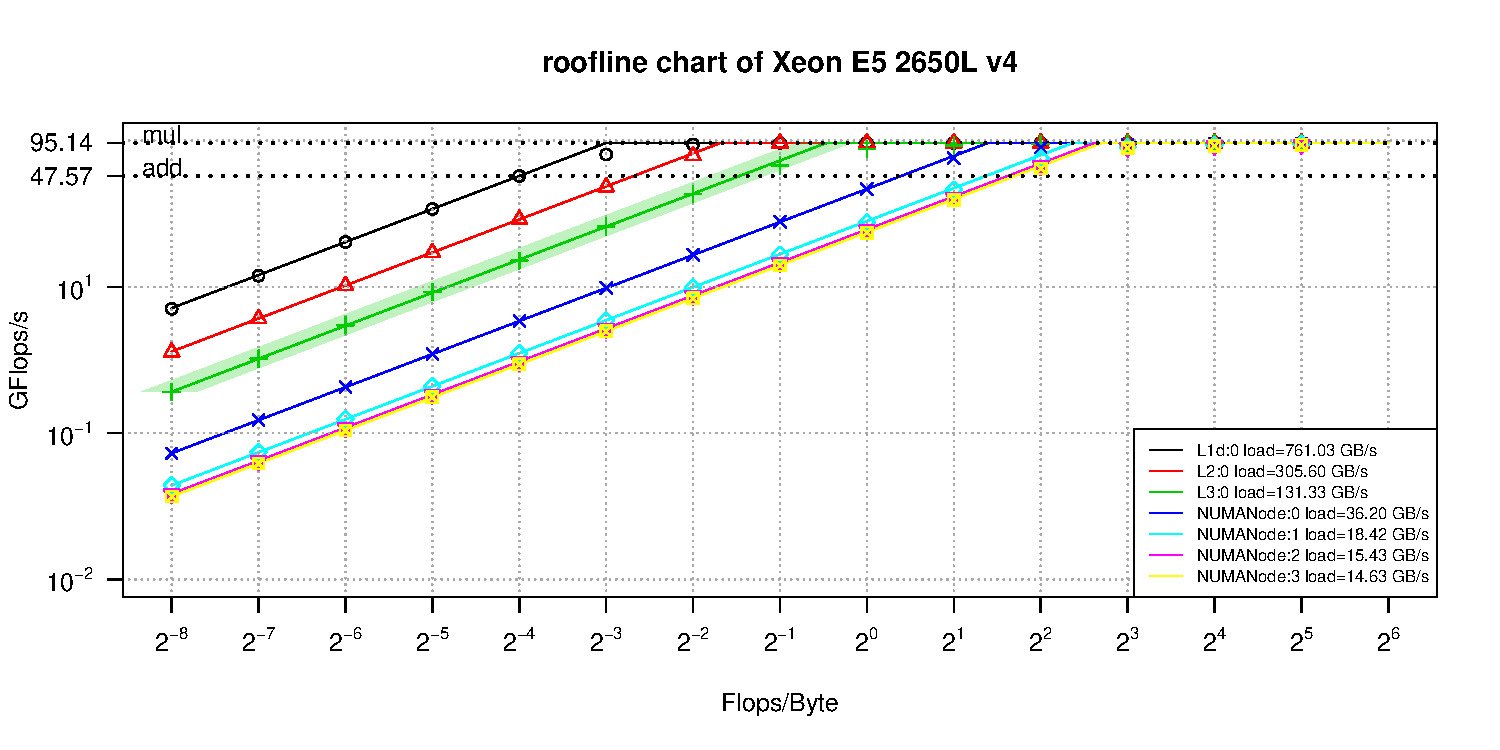
\includegraphics[width=\textwidth]{pictures/roofline_model}
  \caption{The roofline chart on a Xeon E5 2650L v4 processors with 4 NUMA memories spreads on two different packages. On ordinate, the performance is in $10^{^9}$ floating point operations per second. On abscissa, operational intensity is the number of floating point operations per bytes loaded.}
  \label{fig:orig_model}
\end{figure*}

In our contribution, we developped micro-benchmarks for rooflines and their validation, compatible with intel chips.
In this section we take a deep dive into architectures sepcificities, that lead model design choices.

\paragraph{Intra Core specific aspects}
Processors usually implement vector operations, also named Single Instruction Multiple Data~(SIMD) operations.
Depending on the architecture, we pick the operation able to perform on the largest possible vector. Those operation exists
both for compute operations and memory transactions, and multiply the achievable performance of each involved units by the vector
size. By compiling the benchmarks on target architecture, we ensure that largest vector size will be used for the benchmarks.

Moreover, there are several types of memory/compute intructions available on processors, they implement in hardware usual
operations, and yields different throughput. For instance a core may compute multiplications~(mul) and an additions~(add) on
separate FPUs and may also be able to overlap those operations when they do not have dependencies. In this case, the
Core\footnote{smallest execution entity} can double its performance if the code is able to interleave its add and mul operation
that do not have dependency. This principle also applies to memory since some architectures' Cores have 2 channels for load
intructions and 1 for store instructions. Finally, two types of instructions with the same results can have different throughput.
Both architecture design are pictured on figure~\ref{fig:unicore}.
For instance streaming stores will bypass caches to write to memory whereas classic stores will write in the first level cache and
let the hardware replacement protocol handle write back to memory.
Our tool proposes several types of usual operations to benchmark the platform according to applications characteristics.
We can find several arithmetic floating point operation peaks (addition, multiplication, overlapping multiply add, and fuse
multiply add), as well as several bandwidth types (load, store, non temporal load, non temporal store, interleaving of 2 loads and one store), and for several memory levels (L1, L2, L3, (caches \dots), NUMA memories, MCDRAM \dots) detectable with hwloc~\cite{6903671} library.

Since processors have multiple Cores and complex memory hierarchy, several benchmarks scenari may be considered.
We will first describe the sequential scenario we use, then the parallel scenario for platform benchmarking.

\paragraph{Memory Benchmark for Uni-Core Architecture}
\begin{figure}
  \centering
  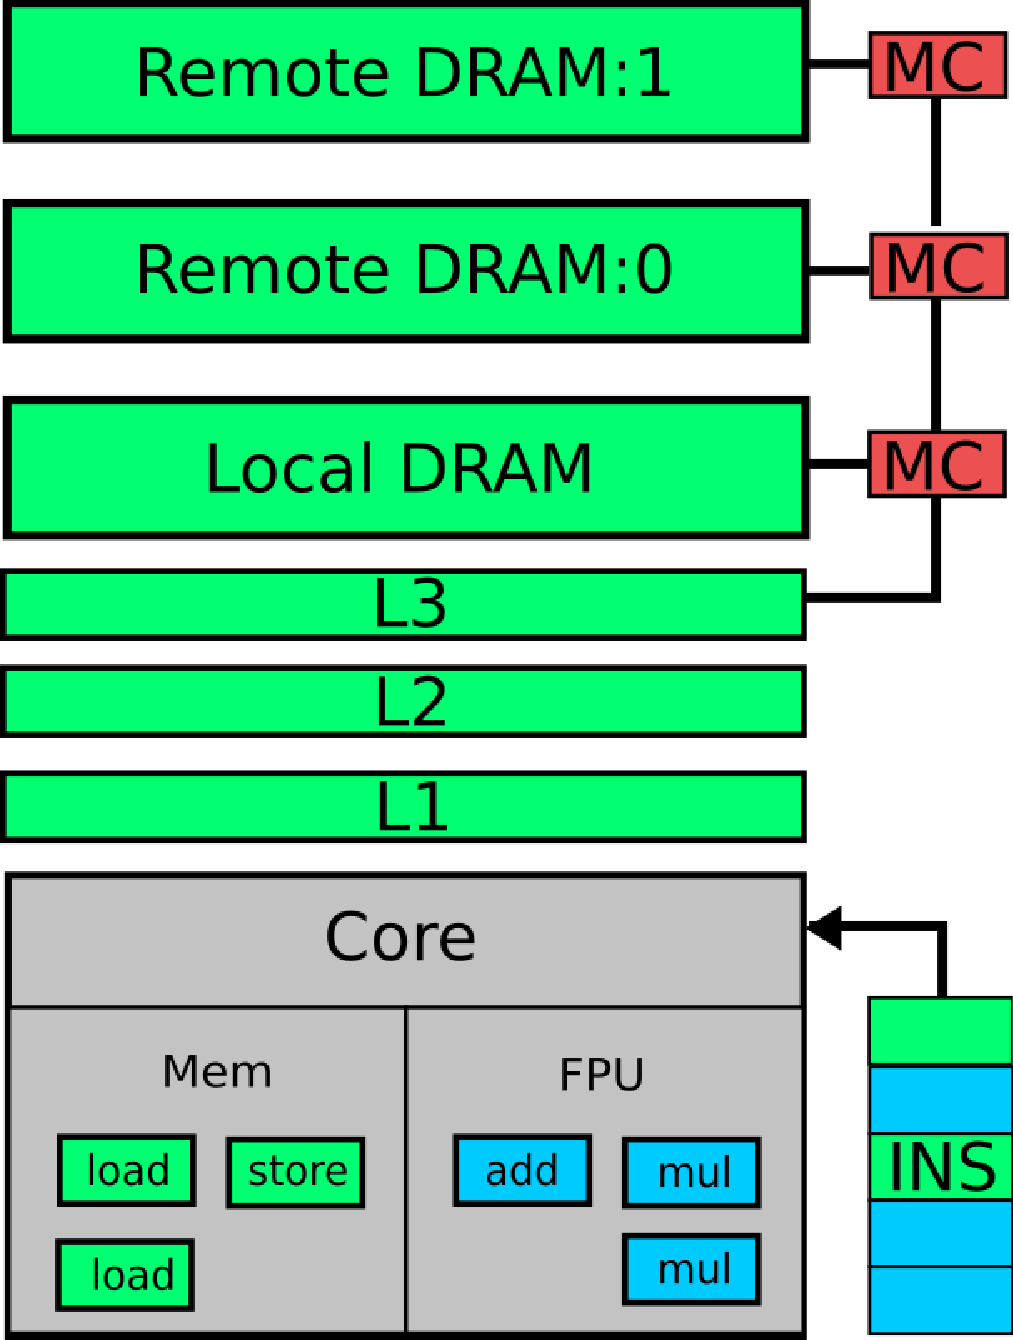
\includegraphics[width=.25\textwidth]{pictures/unicore}
  \caption{Uni-Core machine topology. MC refers as the memory controller. INS refers as the instruction cache.}
  \label{fig:unicore}
\end{figure}

Both the Roofline Model and The Cache Aware Roofline model are single threaded models.
From the Core to the DRAM memory, the memory subsystem is a stack of memories of increasing sizes from bottom to top.
Our benchmark strategy to benchmark the cache hierarchy will be to perform memory operations on increasing size buffers.

On heterogeneous memory subsystems, the DRAM memory level consists in several memories which are not stacked and do not
overlap. They are linked to the cache stack by a common set of memory controllers. This model representation is given on
figure~\ref{fig:unicore}
At this level, the memory subsystem may be bound, by one memory bandwidth, the interconection network bandwidth,
or the memory controllers bandwidth.
Usually, local memory bandwidth is bound by the sequential accesses to it when only one thread is performing memory transaction,
whereas remote memories bandwidth may be bound by the interconnection network bandwidth or memory bandwidth also.
Splitting data among several memories does not yield a better bandwidth than using the local DRAM only.
Therefore, our strategy to benchmak memories will be to benchmark each memory separately, performing memory operations on a large
enough buffer allocated on target memory.

\paragraph{Memory Benchmark for Multi-Core Architecture}

\begin{figure*}
  \centering
  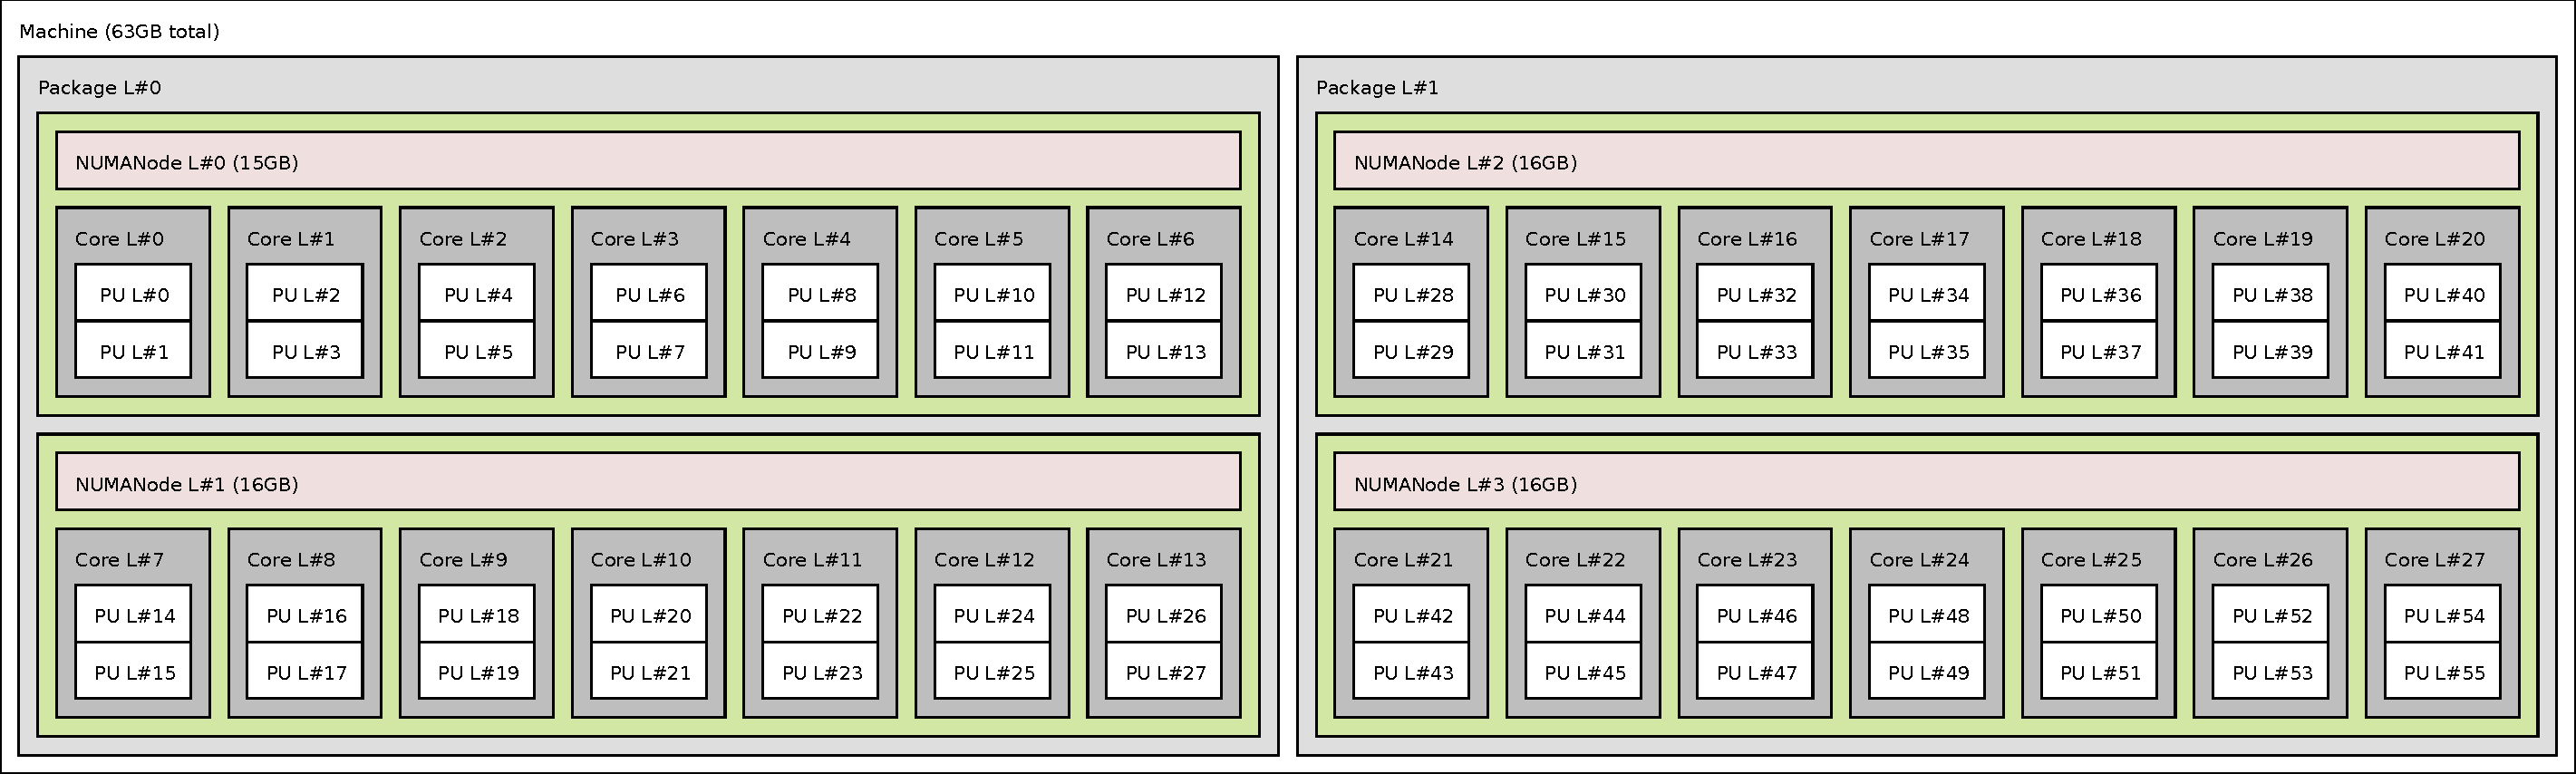
\includegraphics[width=.9\textwidth]{pictures/Xeon_E5_2650L_v4}
  \caption{Xeon E5 2650L v4 topology, without remote nodes' caches and cores, as seen by the benchmark}
  \label{fig:joe0}
\end{figure*}

Figure~\ref{fig:joe0} shows a model of the multi-core architecture we used for our model as given by hwloc.
Nested boxes represent hierarchical inclusiveness of ressources in the machine.
This system is equiped with two blades of two processors each.
In this case the memory bandwidth from two Cores of the same NUMANode to a single memory is the same.
The memory bandwidth of a local memory is now bound by the memory controllers.
It increases when the number of used cores increases but does not scale up to the number of cores on the same chip.
Since the local memory controllers are a bottleneck it does not yields a better bandwidth to use several memories for a
benchmark and it makes sense to benchmark each memory separately.
The choice of the optimal number of threads is not something that cannot be determined analytically and we choose to
set it to the number of Core on the chip (which is not optimal) because applications usually run on full machines.

In brief we set the number of threads to the number of core of a single memory node. Then we run same benchmarks as the sequential
benchmark per thread. Finally we sum the results of each threads.

This is a subjective benchmark from a memory node sight, but since machines with heterogeneous and NUMA memories are symetrics,
it is straightforward that the result will be the same (or a permutation close) from the others nodes sight.

The parallel model representation obtained from machine~\ref{fig:joe0} is shown on figure~\ref{fig:orig_model}.
The system yields a load bandwidth of 761GB/s for the total of its 7 L1 caches per Node, whereas the shared local memory
(NUMANode:0) yields a bandwidth of 36GB/s for the same type of micro-operations.
On figure~\ref{fig:orig_model}, the lines shows the top measures.
One can notice, on L3 a wider line with less opacity showing the measured bandwidth deviation.
For each memory we use different sizes of buffers fitting the memory, and depending on the buffer size, the bandwidth may vary.
We can also notice that for L1 (black line), the points does not stick very well to lines around the ridge. Actually the points
does not measure the bandwidths, but instead validate rooflines. They consist of micro-benchmarks of different known operational
intensities, interleaving memory and compute instruction to reach rooflines, and show how realistic the model is with those
metrics, by measuring each micro-benchmark's performance.

\section{Conclusion and future work}\label{sec:conclusion}
%+++++++++++++++++++++++++++++++++++
In this short paper we prestented the Roofline Model and an extension to heterogeneous memory's sytem using the Cache Aware
Roofline Model methodology. Later on we will validate the interest of this representation with applications. 

\bibliographystyle{plain}
\bibliography{references}

\end{document}
